\documentclass{article}
\usepackage{graphicx}
\usepackage{amsmath}
\usepackage{tikz,pgfplots}
\pgfplotsset{compat=1.18}
\usetikzlibrary{positioning}

\title{Tutorial: Calculating Slopes on Curved Graphs}
\author{Badger Code}
\date{\today}

\begin{document}

\maketitle

\section{Introduction}

In this tutorial, we will learn how to calculate the slope of multiple points on a curved graph. Understanding slopes and tangents is crucial for analyzing the behavior of curves in various fields, including physics and mathematics.

\section{Basic Concepts}

To calculate the slope between points on a curved graph, we need to find the instantaneous rate of change, which corresponds to the slope of the tangent line at a specific point.

\subsection{Tangent Line}

The tangent line touches the curve at a single point and represents the slope at that point. The slope of the tangent line approximates the rate of change of the curve.

\subsection{Derivative}

The derivative of a function provides a general way to calculate the slope of a curve at any point. It is denoted as $f'(x)$ or $\frac{dy}{dx}$.

\section{Calculating the Slope}

Let's go through the step-by-step process of calculating the slope between points on a curved graph using an example.

\subsection{Example}

Consider the function $f(x) = \sqrt{x}$.

\subsubsection{Step 1: Choose Points}

Select two points on the curve, such as $A(4, 2)$ and $B(9, 3)$.

\subsubsection{Step 2: Draw Tangent Line}

Draw the tangent line at point $A$ on the curve.

\begin{center}
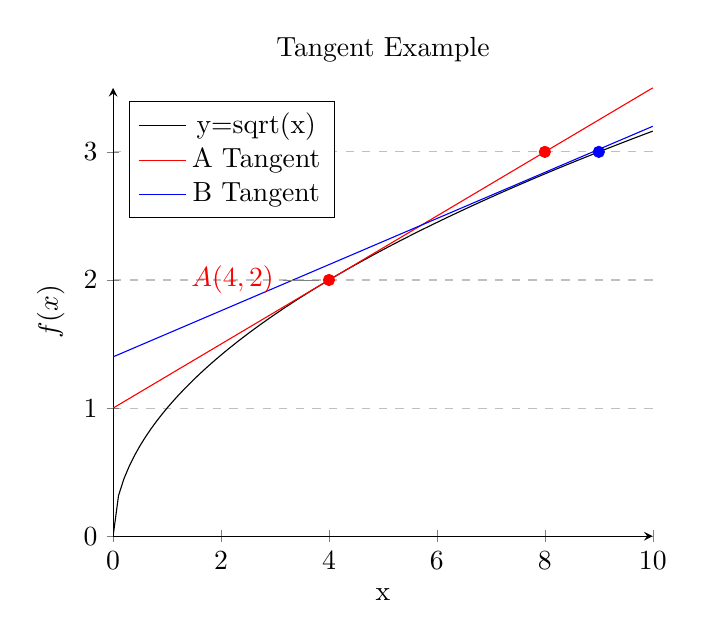
\begin{tikzpicture}
	\begin{axis}[
		title={Tangent Example},
		axis lines=left,
		xlabel={x},
		ylabel={\(f(x)\)},
		legend pos=north west,
		ymajorgrids=true,
		grid style=dashed
	]
		\addplot[
			domain=0:10,
			samples=100,
			color=black
		]
		{sqrt(x)};
		\addlegendentry{y=sqrt(x)}
		\addplot[
			domain=0:10,
			samples=10,
			color=red
		]
		{(.25*x)+1};
		\addlegendentry{A Tangent}
		\addplot[
			domain=0:10,
			samples=10,
			color=blue
		]
		{(.18*x)+1.4};
		\addlegendentry{B Tangent}
		\addplot[color=red,mark=*,only marks] coordinates {
			(4,2)
		}node[pin=180:{$A(4,2)$}]{};
		\addplot[color=red,mark=*,only marks] coordinates {
			(8,3)
		};
		\addplot[color=blue,mark=*,only marks] coordinates {
			(9,3)
		};
	\end{axis}
\end{tikzpicture}
\end{center}

\subsubsection{Step 3: Calculate Slope}

If we follow the A tangent line, we can see that (8,3) is on the tangent line, so we can find the slope(m) of the tangent line with $m=\frac{\Delta{y}}{\Delta{x}}$. \\
$m=\frac{3-2}{8-4}$ \\
$m=\frac{1}{4}$ \\

The derivative of the function is $f'(x) = \frac{1}{2\sqrt{x}}$.

Substitute the x-coordinate of point $A$: $f'(4) = \frac{1}{2\sqrt{4}} = \frac{1}{4}$.

The slope at point $A$ is $\frac{1}{4}$.

\section{Conclusion}

Calculating the slope between points on a curved graph involves approximating the tangent line and using the derivative to find the rate of change at a specific point. This process is fundamental for analyzing the behavior of curves in various contexts. \\

Understanding how to calculate slopes on curved graphs is essential for interpreting the behavior of functions in physics, mathematics, and other disciplines. The concepts of tangents, derivatives, and instantaneous rates of change provide valuable insights into the dynamics of curves.

\end{document}